\begin{figure}[ht]
\vskip 0.2in
\begin{center}
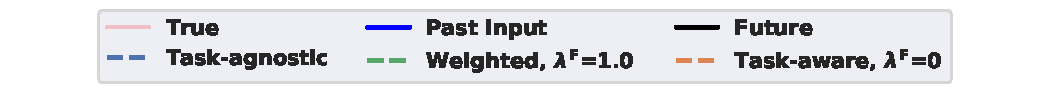
\includegraphics[width=0.8\columnwidth]{figures/forecast_legend.pdf}

\subfigure{
{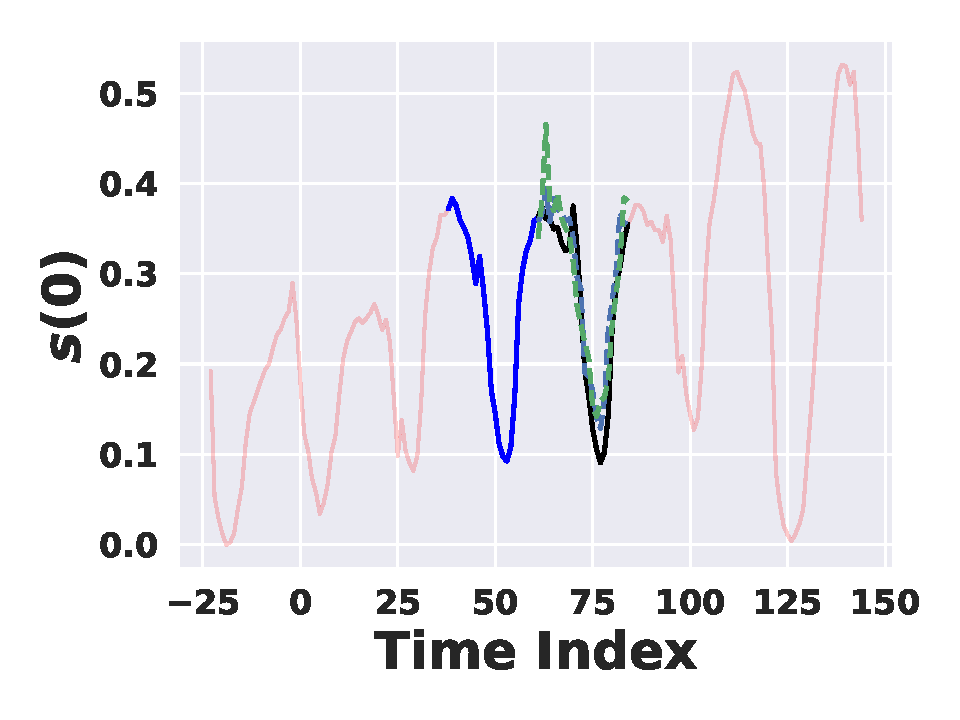
\includegraphics[width=0.4\columnwidth]{figures/appendix/pjm/z_9/forecasts_no_task_aware_sample_1_time_84_signal_0.pdf}}
}
\subfigure{
{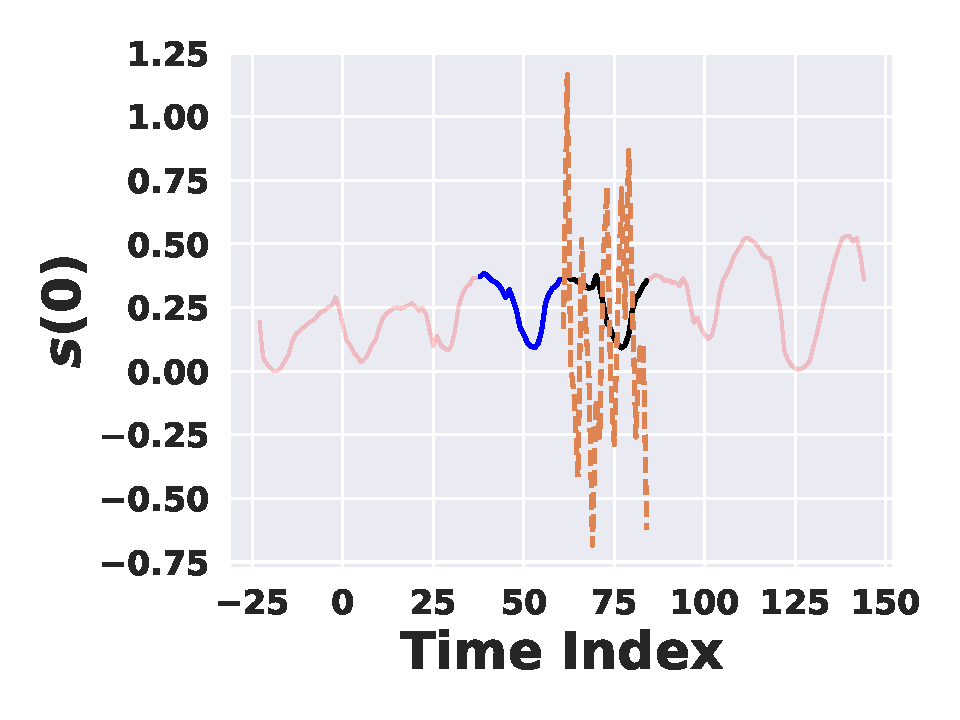
\includegraphics[width=0.4\columnwidth]{figures/appendix/pjm/z_9/forecasts_task_aware_sample_1_time_84_signal_0.pdf}}
}
\caption{\textbf{Forecast comparison: task-agnostic/weighted schemes vs. task-aware scheme.}  Example forecasts for the battery charging scenario at $t=84$ when $Z=9$, for both our task-agnostic/weighted schemes (left) and the task-aware scheme (right). Clearly, a fully task-aware approach with $\lambdaforecast = 0$ yields poor predictions since it does not regularize for prediction errors. This motivates our weighted co-design approach on the left.}
\label{fig:forecasts_comparison}
\end{center}
\vskip -0.2in
\end{figure}

\begin{figure}[ht]
\vskip 0.2in
\begin{center}

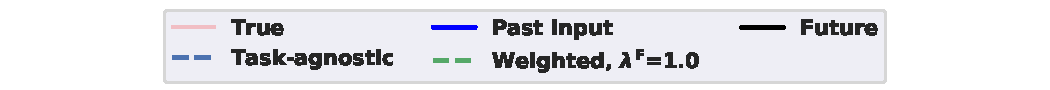
\includegraphics[width=0.8\columnwidth]{figures/forecast_legend_short.pdf}

\subfigure{
{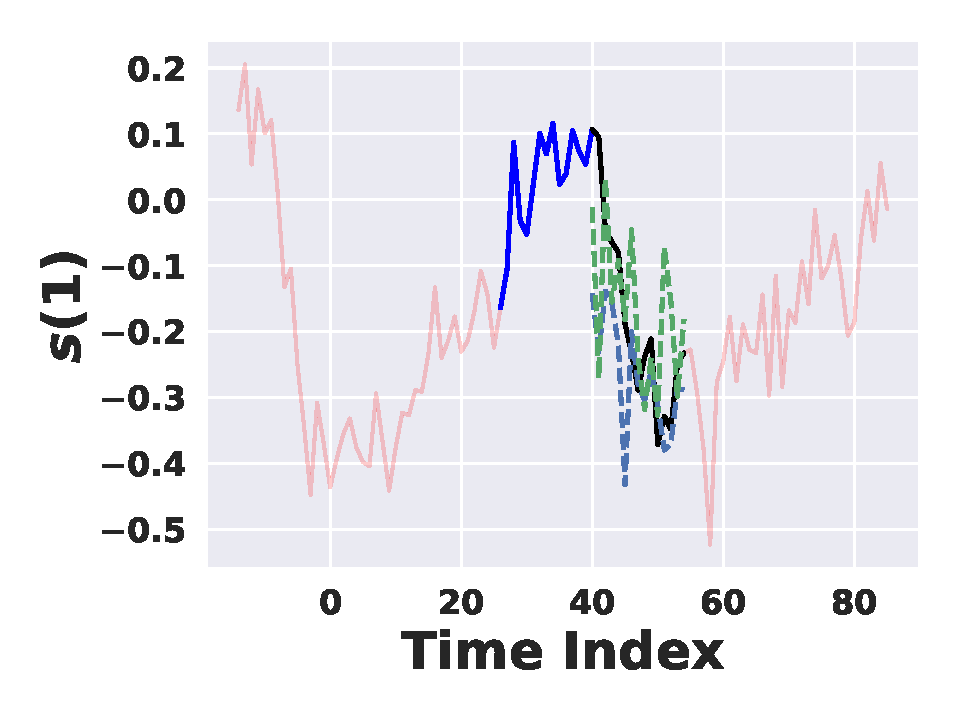
\includegraphics[width=0.4\columnwidth]{figures/appendix/iot/z_4/forecasts_no_task_aware_sample_15_time_54_signal_1.pdf}}
}
\subfigure{
{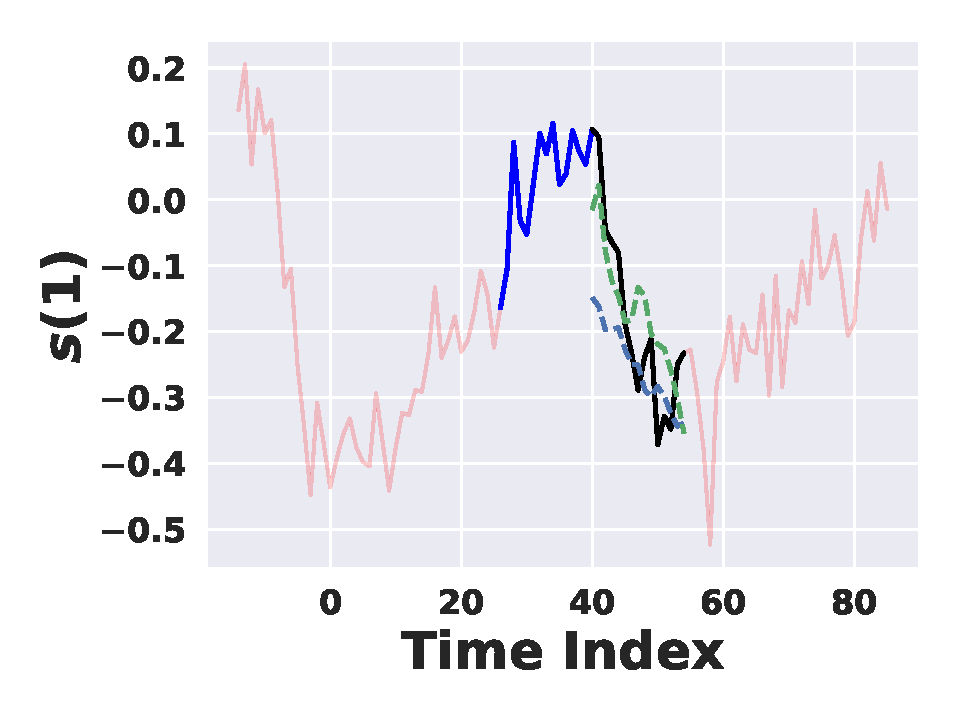
\includegraphics[width=0.4\columnwidth]{figures/appendix/iot/z_9/forecasts_no_task_aware_sample_15_time_54_signal_1.pdf}}
}
\subfigure{
{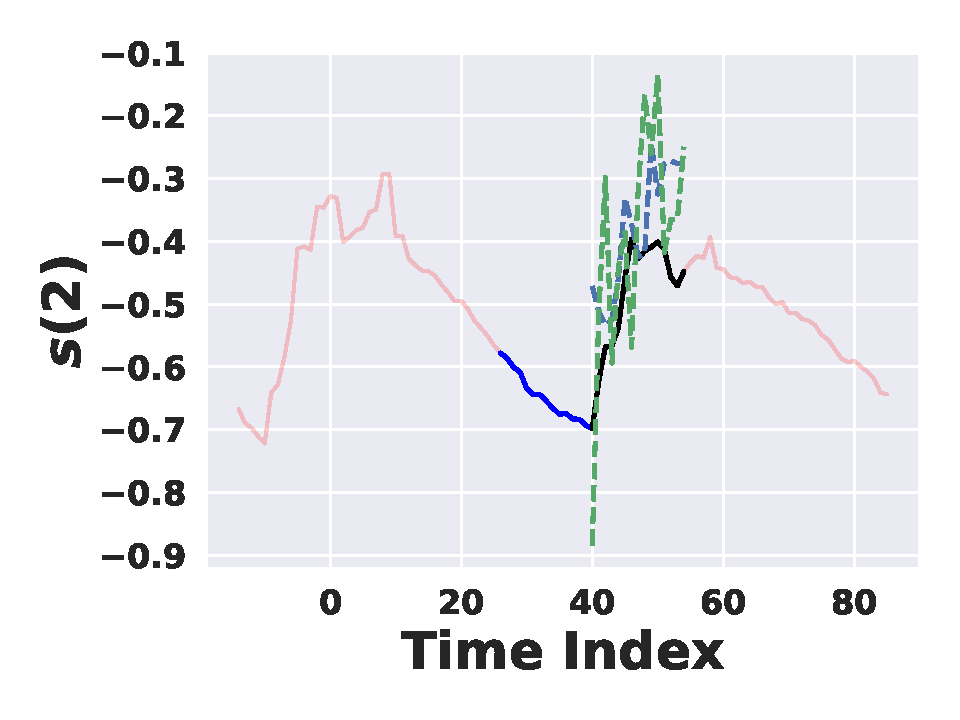
\includegraphics[width=0.4\columnwidth]{figures/appendix/iot/z_4/forecasts_no_task_aware_sample_15_time_54_signal_2.pdf}}
}
\subfigure{
{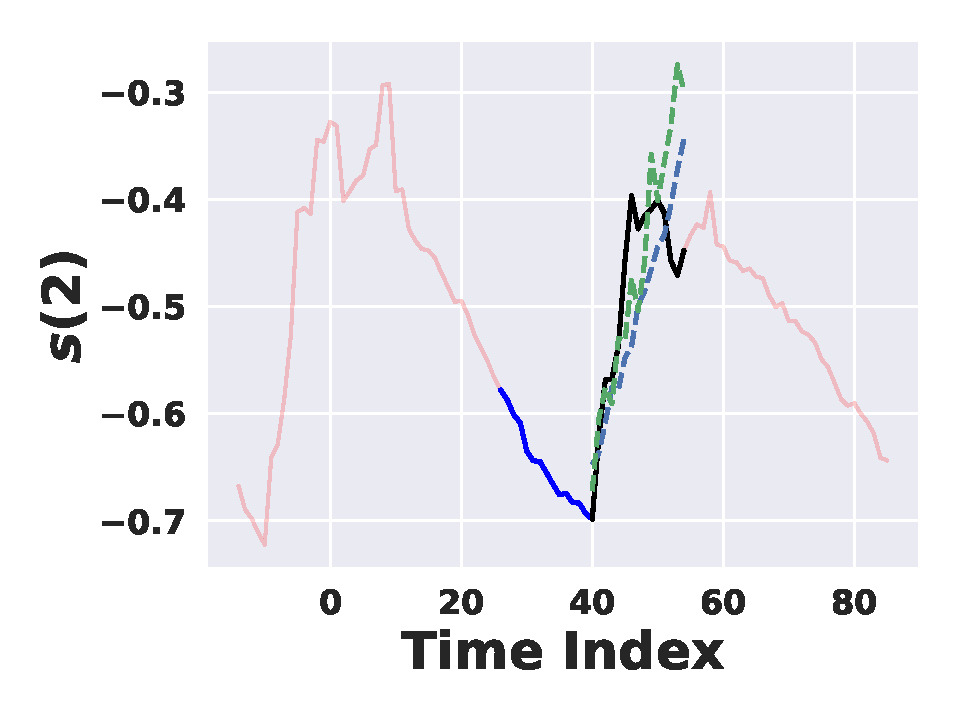
\includegraphics[width=0.4\columnwidth]{figures/appendix/iot/z_9/forecasts_no_task_aware_sample_15_time_54_signal_2.pdf}}
}

\caption{\textbf{Example forecasts (IoT sensors).}  Example forecasts at $t=40$ when $Z=4$ (left) and $Z=9$ (right). 
Clearly, the predictions are more accurate and smooth when $Z=9$. However, with a smaller bottleneck of $Z=4$ (left), we achieve near-optimal control performance since we capture task-relevant features with a coarse forecast that captures high-level, but salient, trends.}
\label{fig:iot_forecasts}
\end{center}
\vskip -0.2in
\end{figure}

\begin{figure}[ht]
\vskip 0.2in
\begin{center}

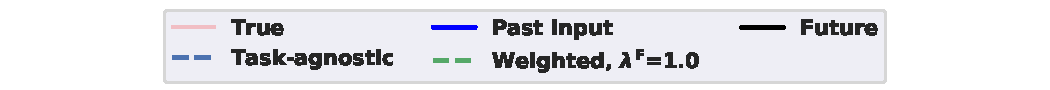
\includegraphics[width=0.8\columnwidth]{figures/forecast_legend_short.pdf}

\subfigure{
{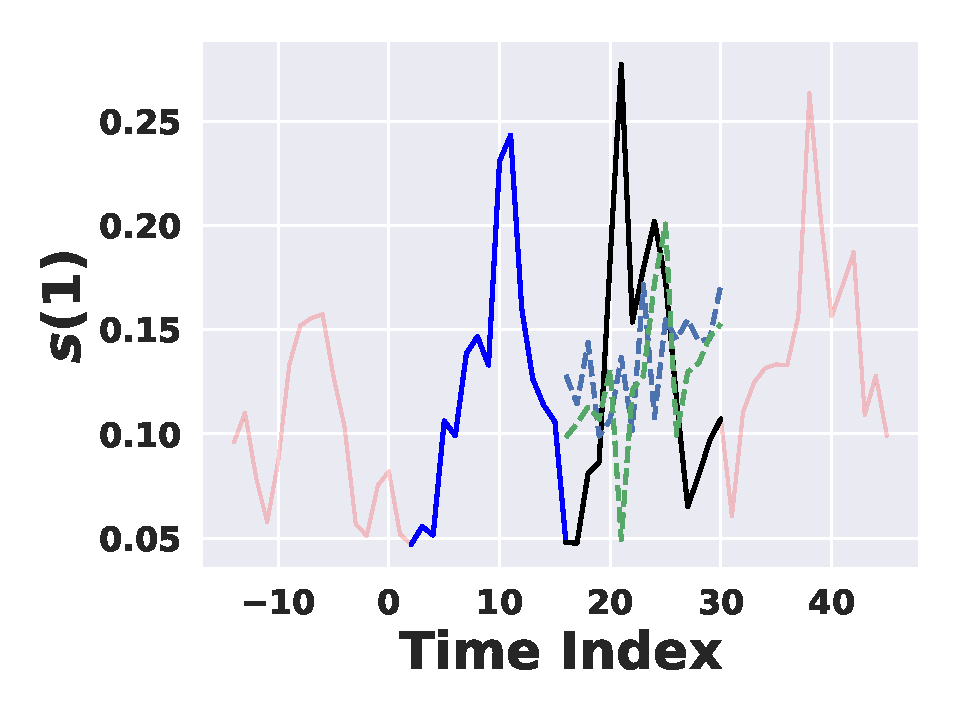
\includegraphics[width=0.4\columnwidth]{figures/appendix/cell/z_4/forecasts_no_task_aware_sample_1_time_30_signal_1.pdf}}
}
\subfigure{
{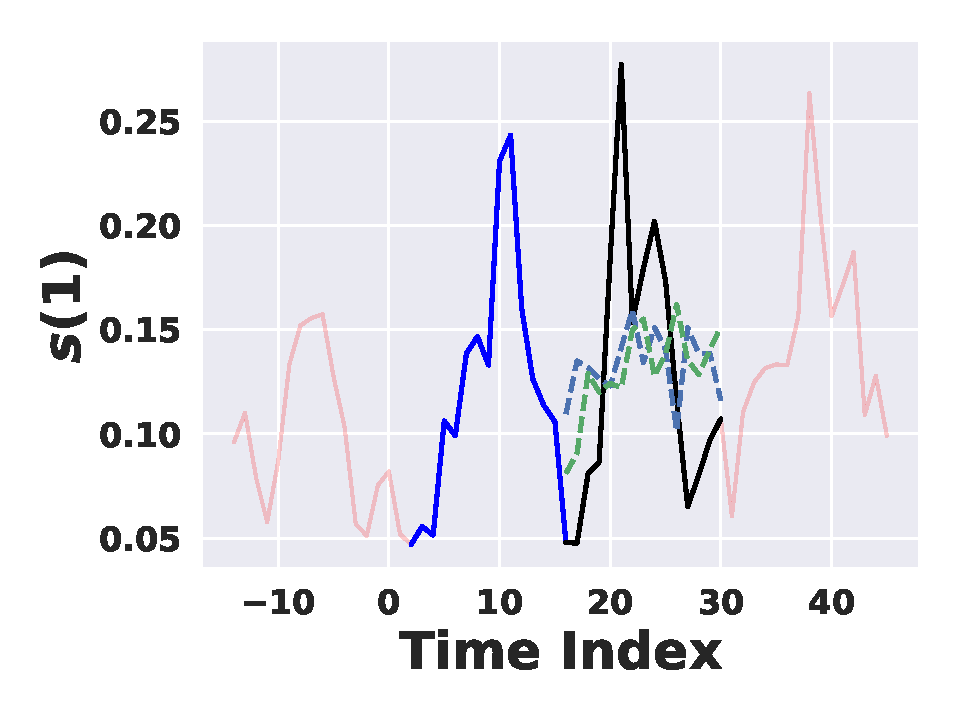
\includegraphics[width=0.4\columnwidth]{figures/appendix/cell/z_9/forecasts_no_task_aware_sample_1_time_30_signal_1.pdf}}
}

\subfigure{
{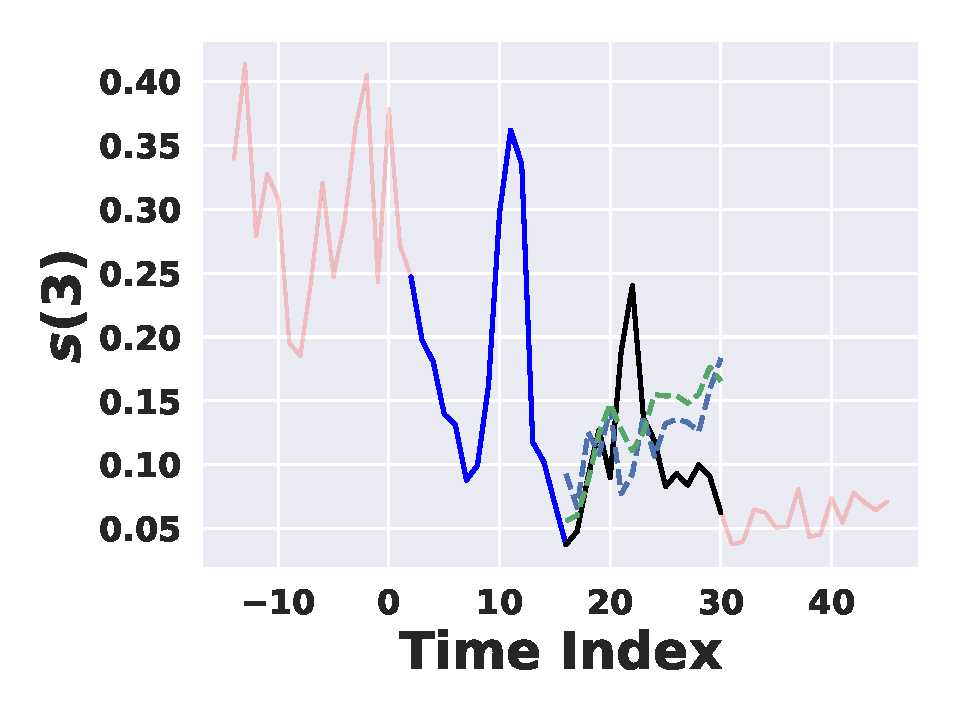
\includegraphics[width=0.4\columnwidth]{figures/appendix/cell/z_4/forecasts_no_task_aware_sample_1_time_30_signal_3.pdf}}
}
\subfigure{
{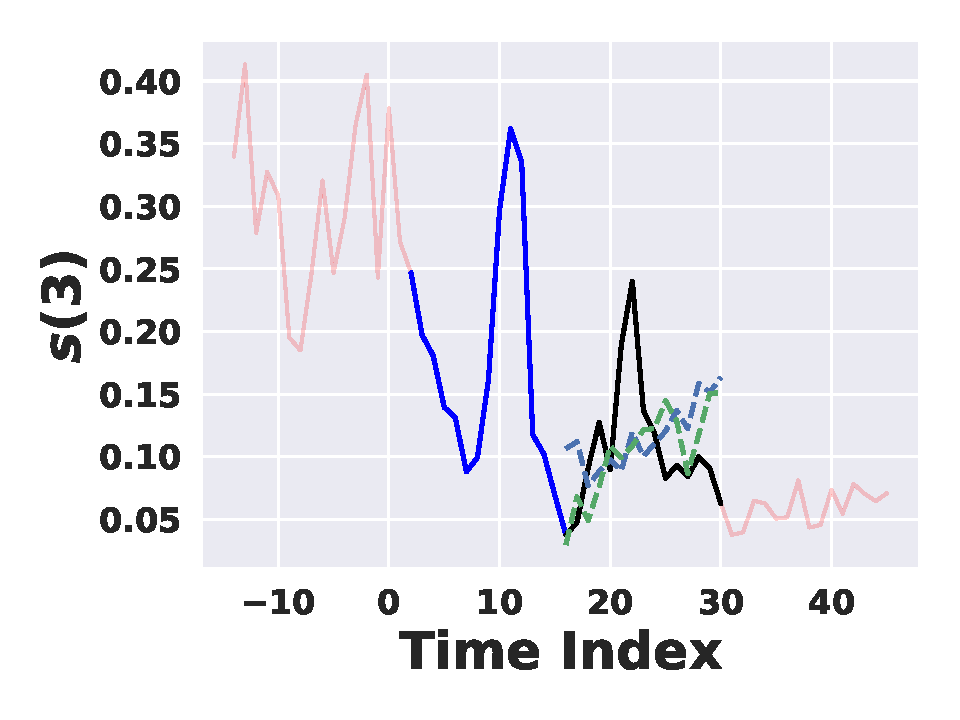
\includegraphics[width=0.4\columnwidth]{figures/appendix/cell/z_9/forecasts_no_task_aware_sample_1_time_30_signal_3.pdf}}
}


\caption{\textbf{Example forecasts (taxi scheduling).}  Example forecasts at of at $t=16$ when $Z=4$ (left) and $Z=9$ (right). This scenario had the worst prediction errors since the cell data is highly stochastic.}
\label{fig:cell_forecasts}
\end{center}
\vskip -0.2in
\end{figure}

\begin{figure}[ht]
\vskip 0.2in
\begin{center}

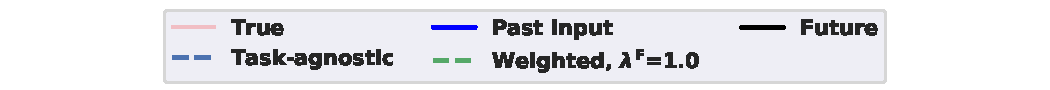
\includegraphics[width=0.8\columnwidth]{figures/forecast_legend_short.pdf}

\subfigure{
{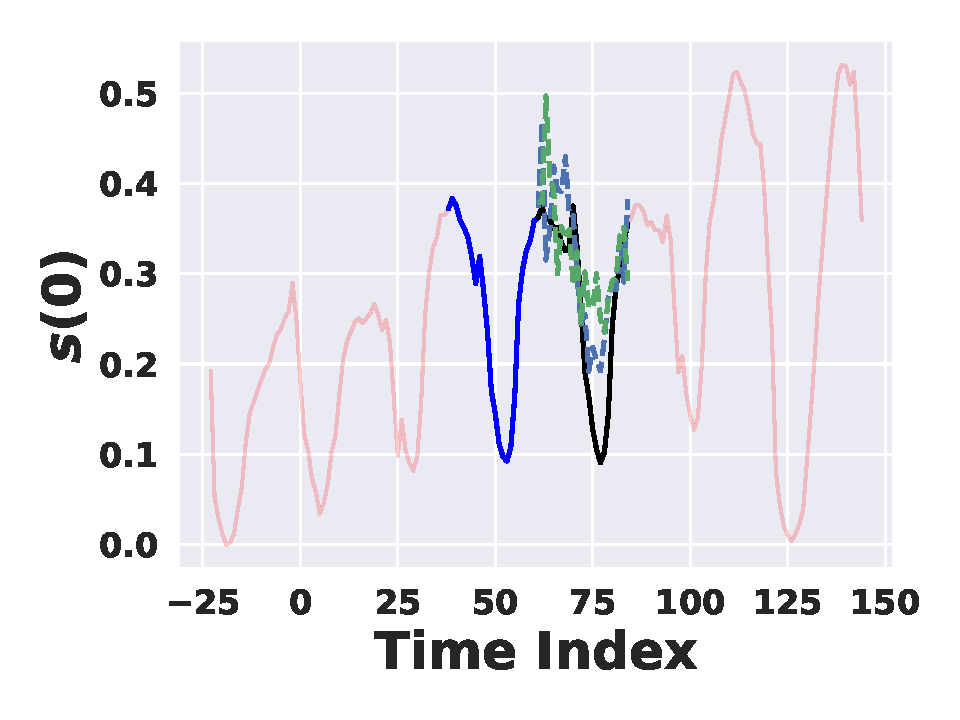
\includegraphics[width=0.4\columnwidth]{figures/appendix/pjm/z_4/forecasts_no_task_aware_sample_1_time_84_signal_0.pdf}}
}
\subfigure{
{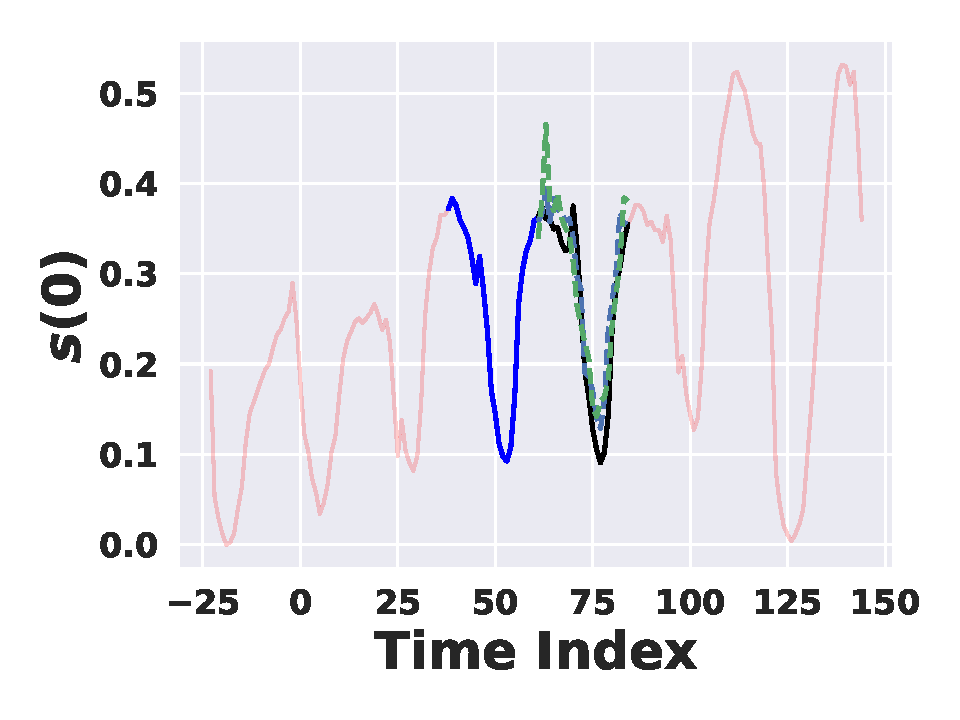
\includegraphics[width=0.4\columnwidth]{figures/appendix/pjm/z_9/forecasts_no_task_aware_sample_1_time_84_signal_0.pdf}}
}
\subfigure{
{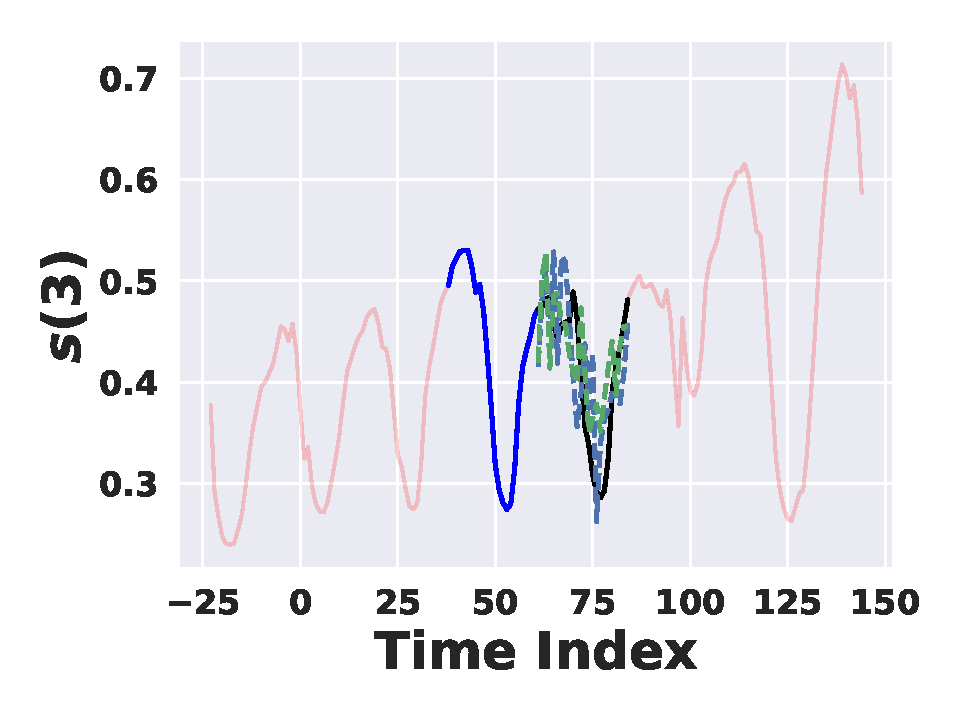
\includegraphics[width=0.4\columnwidth]{figures/appendix/pjm/z_4/forecasts_no_task_aware_sample_1_time_84_signal_3.pdf}}
}
\subfigure{
{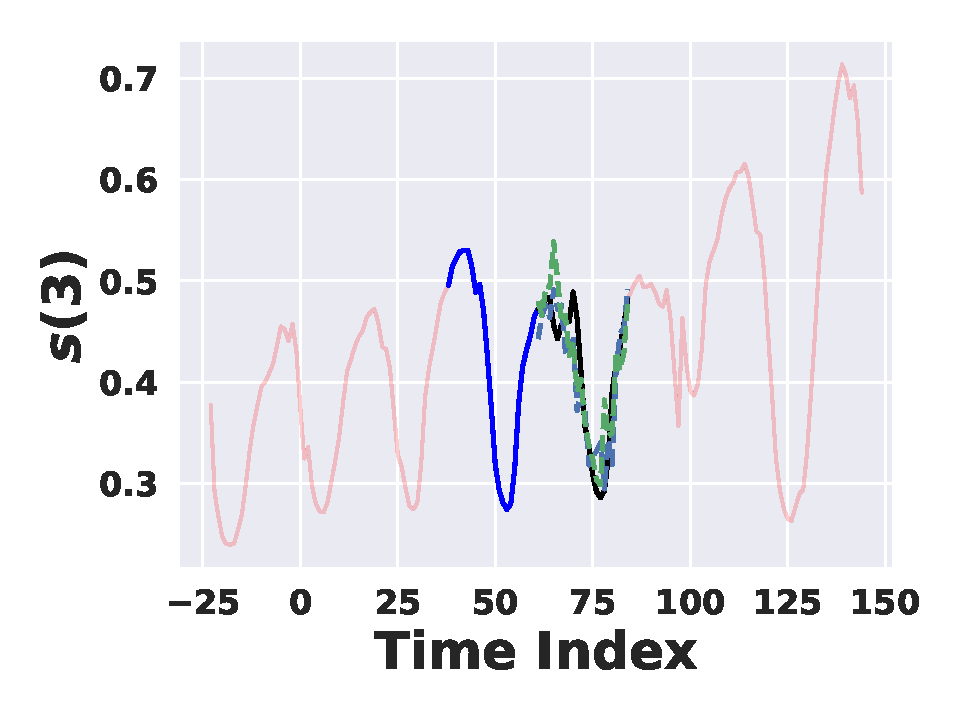
\includegraphics[width=0.4\columnwidth]{figures/appendix/pjm/z_9/forecasts_no_task_aware_sample_1_time_84_signal_3.pdf}}
}

\caption{\textbf{Example forecasts (battery charging).}  Example forecasts at $t=84$ when $Z=4$ (left) and $Z=9$ (right). As before, the predictions are more accurate and smooth when $Z=9$. However, with a smaller bottleneck of $Z=4$ (left), we achieve near-optimal control performance since we capture task-relevant features with a coarse forecast that captures high-level, but salient, trends.}
\label{fig:pjm_forecasts}
\end{center}
\vskip -0.2in
\end{figure}
